\section{IoTサービス}
% (IoTサービスがどのようなもので,どのような背景で登場してきたのか,どんなものがありどのような自動化を図っているのか)}
IoTとは,Internet of Things の略で「モノのインターネット」とも呼ばれる概念である.
IoTでは,様々な物がインターネットにつながり,相互に情報をやり取りすることで,多様な自動化を行う.
IoTサービスとは,ユーザーに対しIoTによる利便性を提供するものである.
\medskip

IoTサービスは,半導体技術の進歩によりコンピューターが小型且つ安価になったこと,通信ネットワークの整備が進み様々な場所から安価に通信が利用可能になったことで登場した.
\medskip

例えば,次のような物がある.
\begin{itemize}
	\item 駐車場の検索・予約・決済サービス\cite{エコパ}
	\item 太陽光発電の監視
\end{itemize}

駐車場の検索・予約・決済サービスとは,ドライバーが空いている駐車場を探す手間を省くためのサービスである.
周囲の空いている駐車場の検索や,予め駐車場を予約しておくことで,駐車場を探す手間を省いている.
このサービスの実現のために,駐車場の駐車スペースにコンピュータを取り付ける.
これらコンピュータが,駐車場が空いているか否か・予約が入っているか否か等をサーバーとやり取りする.
それらにより,サーバーは空いている駐車場の一覧や,利用情報に基づく決済を,ユーザーに提供している.
\medskip

太陽光発電の監視とは,太陽光発電所の発電量や機器の異常を確認しに行くための手間を省くためのサービスである.
このサービスの実現の為に,太陽光発電所の機器にコンピューターを取り付ける.
これらコンピュータが発電量や機器の異常の情報をサーバーとやり取りする.
それにより,サーバーは,発電量や機器の異常をユーザーに知らせる.
\medskip

このように,IoTサービスは,IoT機器とサーバーが連携し,ユーザーに利便性を提供するものである.
今後も数多くサービスが登場すると考えられている.

\section{IoTサービスの構造}
%(IoTサービスの構造要素としてIoT機器とサーバがあること,IoT機器・サーバーとはどのようなものなのか,何をしているのか,その間の通信とはどのようなものなのか)
IoTサービスは,IoT機器とサーバーが連携し利便性を提供するものである.
IoTサービスの構造として,多数のIoT機器とサーバーがインターネットを介し連携する事が挙げられる.
\medskip

\begin{figure}[htbp]
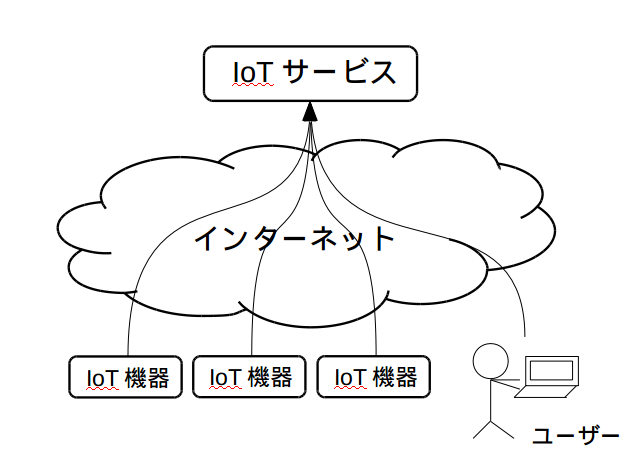
\includegraphics[width=14cm]{images/IoTservice.png}
\caption{IoTサービスの構成図}
\label{fig:IoTservice}
\end{figure}

IoT機器は,様々な環境へ設置され,周囲の状況を検知することや,周囲へなんらかの働きを行う為に使用される.
駐車場の例では,駐車スペースに車が止まっているか否かを検知している.また,予約された駐車スペースであることを別のユーザーへ知らせている.
\medskip

この機器からの情報を収集し,処理しているのがサーバーである.
サーバーは,IoT機器からの情報を蓄積・分析し,IoT機器やユーザーに対し何らかの働きかけを行う.
駐車場の例では,駐車場の利用情報を蓄積・分析し,ユーザーへ対し可視化を行っている.
サーバーにて動作するプログラムが,IoT機器と通信することで,IoTサービスを構成する.
この通信に利用されるのがインターネットである.
様々な通信リンクを用いてIoT機器とサーバー上のプログラムが連携する.
\medskip

このように,IoTサービスの構造は,IoT機器とサーバー上のプログラムがインターネットを介し通信し,連携することで成り立っている.
図\ref{fig:IoTservice}は,IoTサービスの構造図である

\section{IoTサービス維持の問題}
%(IoTサービスの維持の為に何が必要となるのか,それを妨げている物はなんなのか)
IoTサービスは,IoT機器とサーバー上のプログラムがインターネットを介し通信し合うことで成り立っている.
IoTサービスを維持するためには,これらの構造を維持する必要がある.
そのため,IoT機器が正常に動作しているのか,通信が途切れていないか,監視する事が重要である.
ところが,IoT機器が多量に存在することや,IoT機器が接続するネットワークが多様であることから,その監視には技術的困難がある.
また,個別のIoTサービスに組み込まれた監視システム等を別として,一般的な監視サービスも存在しない.
\medskip

IoTサービスでは,多量のIoT機器を使用する.
そのため,個々のIoT機器を識別し,適切に管理することが困難である.
また,家庭内や屋外等,様々な環境下に置かれるIoT機器が接続されるネットワークを予め予期することは困難を極める.
接続先のネットワークでもプライベートアドレスを付与されるなどの他,IoT機器とサーバーとの通信に制限がかかる場合もある.
さらに,IoT機器によっては,移動することを前提とした物もある.
そのような場合,接続されるネットワークが頻繁に切り替わりるため,機器のIPアドレスを利用した既存の機器監視手法は適応することができない.
そのため,遠隔から機器の状態を確認することが難しい.
\medskip

このように,IoTサービスの維持において,IoT機器の動作や通信状態を監視することは重要であるが,その監視には技術的な困難がある.
IoTサービスの円滑な提供や今後の発展の為には,機器が設置されるネットワークに関係なく,機器が多量であっても容易に監視可能な,IoT機器の監視の実現が重要である.


\section{従来の機器監視手法}
\subsection{サーバからの問い合わせによる監視}
	従来から機器監視に用いられてきた手法として,定期的に機器監視サーバから対象機器に状態を問い合わせる手法がある.
	機器監視サーバから,監視対象機器上のエージェントプログラムに,現在の状態を問い合わせる事で機器の監視を実現している.
	\medskip

	この形では,機器監視サーバは,監視対象機器のIPアドレスを覚えておかねばならない.
	そのため,監視対象が接続されるネットワークが切り替わった場合,監視サーバ上に記録されたIPアドレスを変更しなくては監視できない.
	監視対象が,多量且つ移動するIoT機器の監視において,頻繁に監視サーバ上に記録されたIPアドレスを書き換えるのは大変である.
	また,プライベートアドレスの利用時には,サーバーからIoT機器への到達性が失われる可能性がある.

\subsection{監視対象機器からの通知による監視}
	機器監視手法として,定期的に監視対象機器から機器監視サーバーへ状態を送信するという手法がある.
	監視対象機器上のエージェントプログラムが,指定した時間毎に機器監視サーバーへ状態を送信することで,機器の監視を実現している.
	\medskip

	この形だと,機器監視サーバが監視対象のIPアドレスを覚えておく必要がなくなるため,監視対象が接続されるネットワークが切り替わった場合でも,追跡が可能である.
	ところが,エージェントプログラムの導入には,技術スキルと時間が必要である.
	また,サーバーの構築・設定も必要となる.

\subsection{ネットワークによる監視}
	そもそも監視対象機器がつながる為のネットワークを作ってしまおうという動きもある.
	既設の携帯電話網を利用して,IoT機器用ネットワークサービスが展開されている.
	これは,IoT機器向けのデータ通信を提供するサービスで,Web画面から通信量や接続状況を確認することができる.
	携帯電話網を利用しているので,接続状況から機器の状態を推測できる.

	しかし,そのネットワークを利用している場合に限り機器の状況を推測できるので,異なるネットワークに接続された機器と,専用ネットワークを用いた機器とを1箇所で監視することが難しい.

\subsection{既存手法のまとめ}
	既存の手法として,サーバーからの問い合わせによる監視,監視対象機器からの通知による監視,ネットワークによる監視といった手法がある.
%	サーバーからの問い合わせによる監視は,現実的でなく,







\section{岡本商店街での事例}
2015年12月8日から2016年2月26日まで、NPO法人コミュニティリンクへのインターンシップの一環として、実験を行った。
人流観測を行い、結果を分析し商店街の活性化に役立てるという趣旨で行った。
人流観測は、2016年2月7日から2016年3月14日まで行った。
岡本商店街とは、神戸市東灘区にある阪急岡本駅とJR摂津本山駅の間にある商店街のことである。

人流観測とは、各地点から各地点迄をある時に移動した人数を観測するものである。
通常は、観察員がカウンタを用いて数えるが、それでは各地点間を移動した人数はわかるが、その人が以前どの地点に居たのかはわからない。
そこで、携帯電話についているWifi機能を利用し、観測を行うこととした。
携帯電話のWifi機能は、無線LANの接続に使われるが、接続毎にWifi機能を有効にすることが手間なため、常時ONにしている人も少なくない。
携帯電話のWifi機能を有効にしている場合、携帯電話から接続可能な無線LANを探す為、プローブパケットというものが定期的に送出される。
プローブパケットには、そのプローブパケットを送出した機器の物理アドレスが含まれている。
そのプローブパケットを複数地点で観測し、含まれている物理アドレスを照合することで、携帯電話端末を持った人がどのように移動をしたのかが分かる。
岡本商店街では、この原理を利用して、人流観測を行った。

本事例では、岡本商店街の5店舗に開発した観測機器を設置し、サーバにて蓄積・分析・可視化を行った。
開発した観測機器は、RaspberryPiとampsence、rsyncというソフトウェアを利用した。
図\ref{fig:okamoto_pict1}は、開発した観測機器である。
\begin{figure}[htbp]
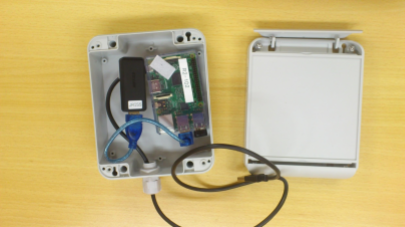
\includegraphics[width=16cm]{images/okamoto_pict1.png}
\caption{岡本商店街人流観測 使用した機器}
\label{fig:okamoto_pict1}
\end{figure}

RaspberryPiとは、小型PCの一つで安価に入手が可能である。
ampsenceとは、プローブパケットを受信しファイルへ記録するソフトウェアである。
図\ref{fig:okamoto_pict2}は、携帯電話と観測機器、サーバーの関係を表している。
\begin{figure}[htbp]
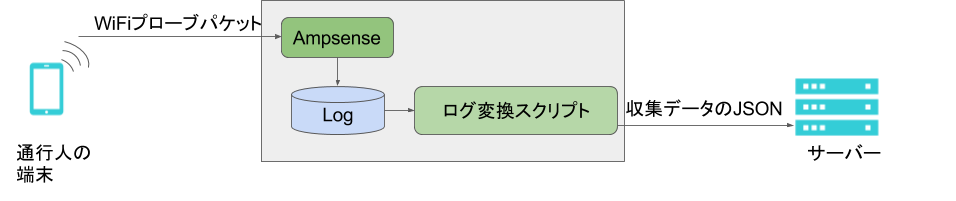
\includegraphics[width=16cm]{images/okamoto_pict2.png}
\caption{岡本商店街人流観測 動作イメージ?}
\label{fig:okamoto_pict2}
\end{figure}

rsyncとは、ディレクトリの中を同期させるプログラムで、遠隔にあるコンピュータの指定したディレクトリの中と、手元のコンピュータの指定したディレクトリを同期することができる。
開発した観測機器では、定期的にrsyncを実行するシェルプログラムを置き、起動時に自動で実行するよう設定した。
それによって、各所に設置された観測機器の情報をサーバー上に集約・蓄積する。
分析・可視化については、Webアプリケーションを作成した。
分析については、作成したプログラムがとりおこない、可視化については、作成したWebアプリケーションが行っている。
図\ref{fig:okamoto_ss}は作成したWebアプリケーションである。
\begin{figure}[htbp]
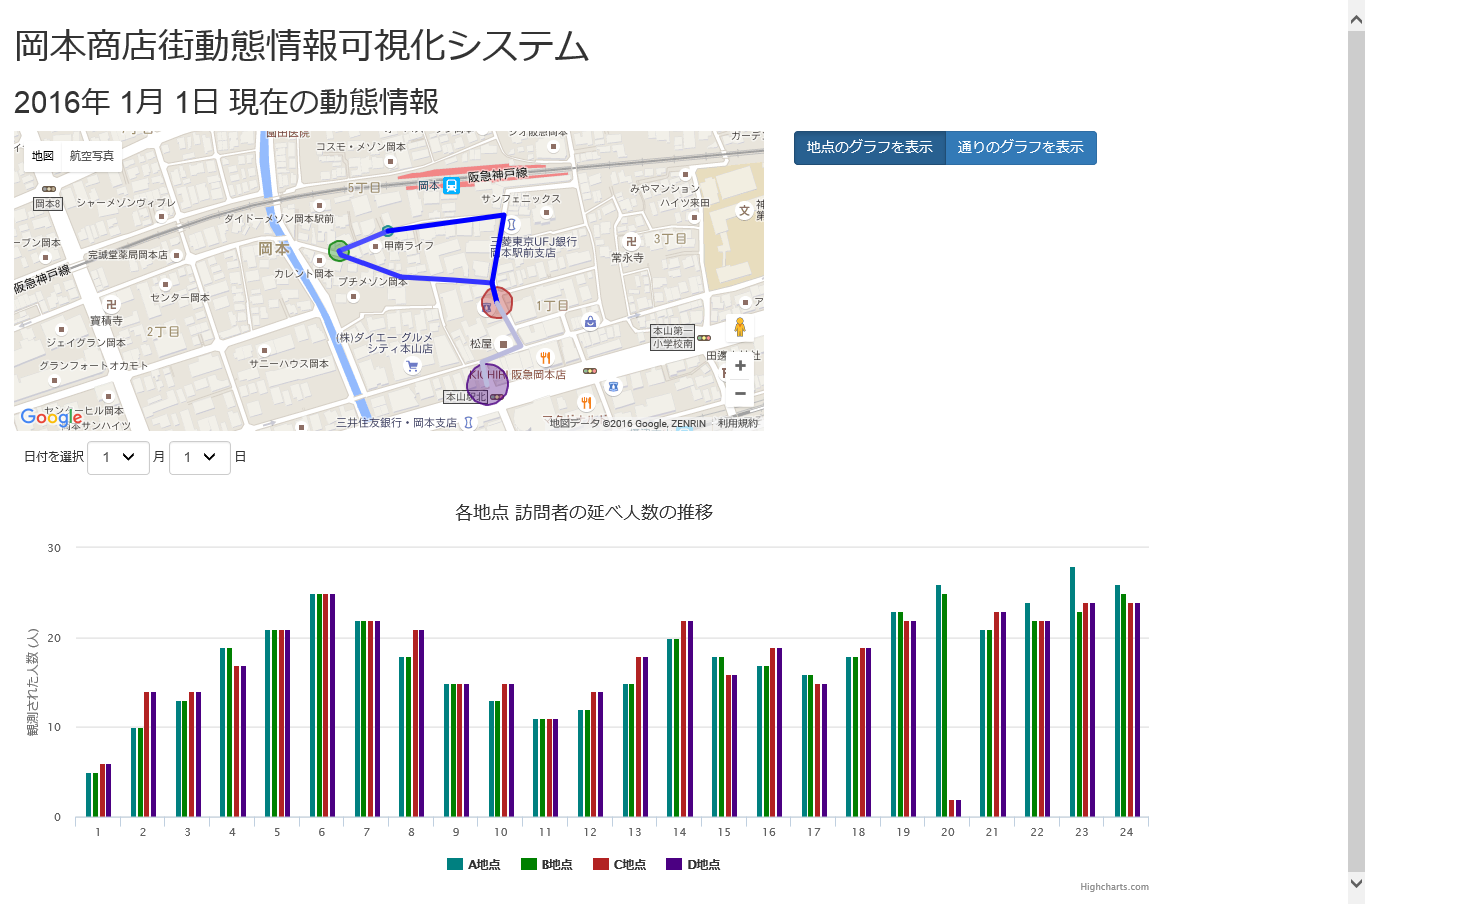
\includegraphics[width=16cm]{images/okamoto_scr1.png}
\caption{岡本商店街人流観測可視化アプリケーションスクリーンショット}
\label{fig:okamoto_ss}
\end{figure}


実験としては、個々のRaspberryPi内に、XX分おきに次のような形式のデータをファイルとして書き出し、定期的に実行されるrsyncによって、サーバー側のディレクトリと個々のRaspberryPiのディレクトリを同期させることで収集した。

ampsenceが書き出すデータは次のような形式の連なりとなっており、XX分おきに新たなファイルとして書き出される。
\begin{lstlisting}
\end{lstlisting}
このようなデータファイルをRaspberryPiに保存し、サーバー側のディレクトリとrsyncを使用して同期することで、データの転送を実現した。

\subsection{実験結果}
2月7日から3月14日の35日間観測を行ったが、全地点で問題なく観測できたのは、18日間だけであった。
図\ref{fig:okamoto_dat1}、図\ref{fig:okamoto_dat2}、図\ref{fig:okamoto_dat3}は、期間中の観測人数の推移を示す。
\begin{figure}[htbp]
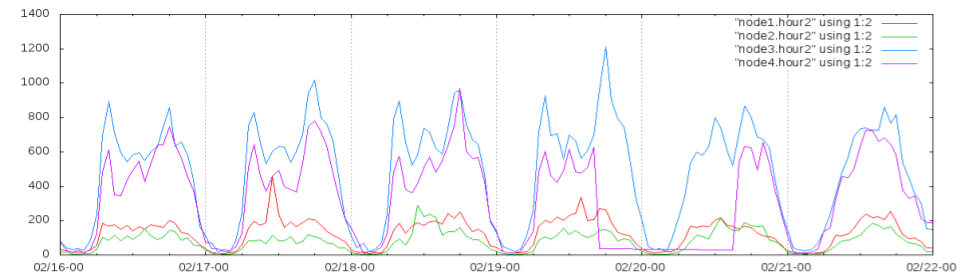
\includegraphics[width=16cm]{images/okamoto_dat1.png}
\caption{岡本商店街人流観測 観測1}
\label{fig:okamoto_dat1}
\end{figure}
\begin{figure}[htbp]
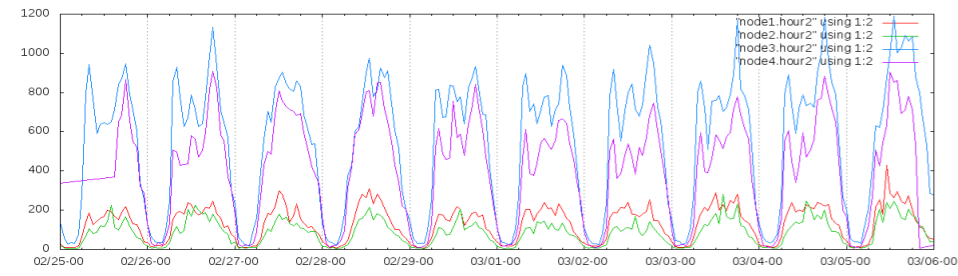
\includegraphics[width=16cm]{images/okamoto_dat2.png}
\caption{岡本商店街人流観測 観測2}
\label{fig:okamoto_dat2}
\end{figure}
\begin{figure}[htbp]
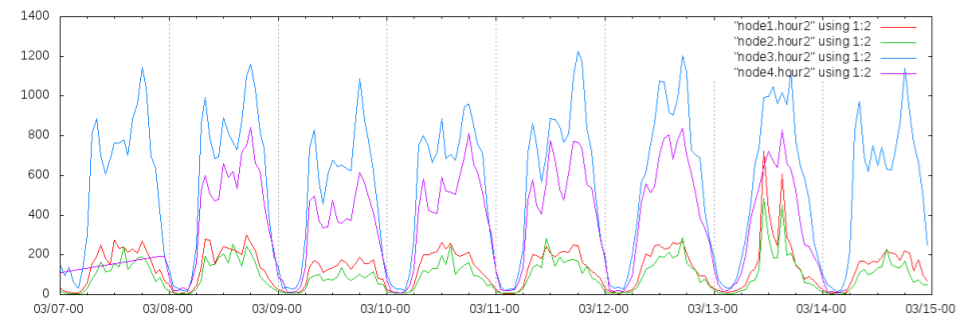
\includegraphics[width=16cm]{images/okamoto_dat3.png}
\caption{岡本商店街人流観測 観測3}
\label{fig:okamoto_dat3}
\end{figure}

この実験を通して、このような結果が得られた。
どのような結果が得られたのか
実験結果
%実験として、どのようなデータをどのように収集して、どのような結果が得られたのか。
%データの形式をはりつけて、コノようなデータですと説明

\subsection{課題点}

しかし、実験を始めると、いくつか不具合が見つかった。
まず、機器がネットワークに繋げていない事があった。
また、機器の電源そのものが入っていない事があった。
そのため、分析が上手く動作せず、可視化が行えない事があった。

機器がネットワークに繋げていない場合、観測データは同期されず、機器内に蓄積されていくことになる。しかし、機器自体は、そもそもインターネットを介してサーバーに順次送信することを想定していたため、蓄積できるスペースは少ない。
こうして溢れてしまった観測データは、蓄積されず捨てられてしまったため、分析の際に観測データが揃わないという自体が発生した。

機器の電源がそもそも入っていなかった場合、そもそも観測することができない。
そのため、分析することもできない。

これら事象が発生した場合、分析アプリケーションでは、何も観測されなかったものとして処理していたため、その分析データを可視化するアプリケーションでは、何も観測されていなかったのか、機器に何か不具合があったのか判断がつきにくかった。

本実験では、定期的に可視化アプリケーションの画面を確認し、他地点では観測されているのに、該当地点では観測されていないと言った場合に、何か不具合があったものとして、現地に赴き対処した。

本実験としては、商店街に報告する義務があったので、実験期間終了後、機器を回収し、機器内に保存されたデータを吸い上げ、分析するという作業をすることで、ある程度は補完できたものの、観測データが存在しない・不十分な曜日や時間帯については分析を行えず、最低限の分析結果しか出すことができなかった。

しかし、各機器の動作状態がすぐに知る事ができれば、夜間等を除き、より良い分析が行えたのではないかと考える。




\section{株式会社SORACOM様へヒアリング}
インターネットへの接続を担う、通信キャリアが行っている機器の監視について調査するために、株式会社SORACOM様を訪問した。
株式会社SORACOM様とは、IoTプラットフォームとして、IoT機器の通信からクラウドまでの接続を提供している会社である。

株式会社SORACOM様では、IoT機器向けのインターネット接続サービス「SORACOM Air」を提供している。SORACOM Airでは、SIMカードを利用した通信を使用している。
そのため、個々の機器をSIMカードに個別に振られたIDによって識別可能である。
また、どのSIMカードが基地局と通信を行っているのかを見ることで、簡易ながらもIoT機器が動作している事を確認することができる。

しかし、監視にはSORACOM Airを利用していなければならず、また、他のネットワークで稼働している機器の状態をSORACOMが提供するインターフェースで見ることも出来ない。要は、複数のネットワークを利用してIoTを構築している場合、一箇所でまとめて見ることが出来ないという利便性の問題がある。



\section{株式会社ルナネクサス様へ聞き取り}
IoT機器の監視が重要であること、監視にて困っている事、また監視システムには何が必要なのかを探るため、太陽光発電所へIoT機器を販売している株式会社ルナネクサス様を訪問した。

株式会社ルナネクサス様では、太陽光発電事業を展開している事業主に対し、発電量や発電に係る機器の状態を遠隔から監視できるIoTサービスを展開している。
独自に開発したIoT機器を発電に係る機器に取り付け、SORACOM Airというインターネット接続サービスを使用して、機器からの情報をサーバーへ蓄積し、ユーザーへ提供している。
SORACOM Airとは、後術するIoT機器向けのインターネット接続サービスの事である。

太陽光発電に係る機器は、通常発電所のわきに小さなプレハブを建て、その中に設置する。
太陽光発電所は日当たりが良いため、夏場、プレハブの中は太陽の熱と機器が発する熱で60度を超える。
そのため、機器が正常に動作しているかどうかを監視する必要がある。

